\documentclass{article}

% Setting
\usepackage{fouriernc}
\usepackage[T1]{fontenc}

% Formatting
\setlength{\parskip}{5pt}
\setlength{\parindent}{0pt}

% Text

% Math
\usepackage{mathtools, amssymb, bm, amsthm, amsthm}
\usepackage{bbm}
% original mathcal
\DeclareMathAlphabet{\mathcal}{OMS}{zplm}{m}{n}

% Math Theorem

% Math Shortcut
\DeclareMathOperator{\sign}{sgn}
\DeclareMathOperator{\samax}{softargmax}
\DeclareMathOperator{\smax}{softmax}
\DeclareMathOperator{\smin}{softmin}
\DeclareMathOperator{\diag}{diag}
\DeclareMathOperator*{\argmax}{\arg\max}
\DeclareMathOperator*{\argmin}{\arg\min}
\DeclareMathOperator{\sech}{sech}
\newcommand{\matr}[1]{{#1}}     % ISO complying version
\newcommand{\vect}[1]{{#1}}     % ISO complying version

% Number sets
\newcommand{\N}{\mathbb{N}} % Natural Numbers
\newcommand{\Z}{\mathbb{Z}} % Integers
\newcommand{\Q}{\mathbb{Q}} % Quotient
\newcommand{\R}{\mathbb{R}}	% Real Numbers
\newcommand{\E}{\mathbb{E}}	% Real Numbers
% \newcommand{\C}{\mathbb{C}} % Complex Numbers

% ML
\newcommand{\cL}{\mathcal{L}}
\newcommand{\cN}{\mathcal{N}}

\newcommand{\vx}{{x}}
\newcommand{\vy}{{y}}
\newcommand{\vb}{{b}}
\newcommand{\vz}{{z}}
\newcommand{\mW}{{W}}


\usepackage{hyperref}
\hypersetup{
    colorlinks=true,
    linkcolor=blue,
    filecolor=magenta,      
    urlcolor=cyan,
}
%Algorithm
\usepackage[ruled,vlined]{algorithm2e}
% Other
\usepackage[shortlabels]{enumitem}
\usepackage{cleveref}
\usepackage{xcolor}
\usepackage[]{tcolorbox}
\usepackage{listings}
\usepackage{graphicx} 





\title{Homework 1: Backpropagation}
\author{CSCI-GA 2572 Deep Learning}
\date{Fall 2024}

\begin{document}

\maketitle

%%%%%%%%%%%%%%%%%%%%%%%%%%%%%%%%%%%%%%%%%%%%%%%%%%%%%%%%%%%%%%%%%%%%
%%%%%%%%%%%%%%%%%%%%%%%%%%%%%%%%%%%%%%%%%%%%%%%%%%%%%%%%%%%%%%%%%%%%
%%%%%%%%%%%%%%%%%%%%%%%%%%%%%%%%%%%%%%%%%%%%%%%%%%%%%%%%%%%%%%%%%%%%
The goal of homework 1 is to help you understand the common techniques used in
Deep Learning and how to update network parameters by the using backpropagation
algorithm.

Part 1 has two sub-parts, 1.1, 1.2, 1.3 majorly deal with the theory of
backpropagation algorithm whereas 1.4 is to test conceptual knowledge on deep
learning. For part 1.2 and 1.3, you need to answer the questions with
mathematical equations. You should put all your answers in a PDF file and we
will not accept any scanned hand-written answers. It is recommended to use
\LaTeX.

For part 2, you need to program in Python. It requires you to implement your
own forward and backward pass without using autograd. You need to submit your
$\texttt{mlp.py}$ file for this part.

The due date of homework 1 is $\texttt{23:55 EST}$ of $\texttt{09/22}$. Submit
the following files in a zip file $\texttt{your\_net\_id.zip}$ through
\href{https://www.gradescope.com}{Gradescope} (Gradescope can be either
accessed through Brightspace course page --> Content or you should've received
an email from Gradescope for log-in instruction):
\begin{itemize}
  \item $\texttt{theory.pdf}$
  \item $\texttt{mlp.py}$
  \item $\texttt{gd.py}$
\end{itemize}

The following behaviors will result in penalty of your final score:
\begin{enumerate}
  \item 5\% penalty for submitting your files without using the correct format. (including naming the zip file, PDF file or python file wrong, or adding extra files in the zip folder, like the testing scripts from part 2).
  \item 20\% penalty for late submission within the first 24 hours. We will not accept any late submission after the first 24 hours.
  \item 20\% penalty for code submission that cannot be executed using the steps we mentioned in part 2.
        So please test your code before submit it.
\end{enumerate}

\newpage

%%%%%%%%%%%%%%%%%%%%%%%%%%%%%%%%%%%%%%%%%%%%%%%%%%%%%%%%%%%%%%%%%%%%
%%%%%%%%%%%%%%%%%%%%%%%%%%%%%%%%%%%%%%%%%%%%%%%%%%%%%%%%%%%%%%%%%%%%
%%%%%%%%%%%%%%%%%%%%%%%%%%%%%%%%%%%%%%%%%%%%%%%%%%%%%%%%%%%%%%%%%%%%
\section{Theory (50pt)}

To answer questions in this part, you need some basic knowledge of linear
algebra and matrix calculus. Also, you need to follow the instructions:
\begin{enumerate}
  \item Every provided vector is treated as column vector.
  \item IMPORTANT: You need to use the numerator-layout notation for matrix calculus.
        Please refer to
        \href{https://en.wikipedia.org/wiki/Matrix_calculus#Numerator-layout_notation}{Wikipedia}
        about the notation. Specifically, $\frac{\partial{y}}{\partial{\mathbf{x}}}$ is
        a row-vector whereas $\frac{\partial{\mathbf{y}}}{\partial{x}}$ is a
        column-vector
  \item You are only allowed to use vector and matrix. You cannot use tensor in any of
        your answer.
  \item Missing transpose are considered as wrong answer.
\end{enumerate}

\subsection{Two-Layer Neural Nets}

You are given the following neural net architecture:
%
\[
  \texttt{Linear}_1 \to f \to \texttt{Linear}_2 \to g
\]
%
where $\texttt{Linear}_i (x) = \bm{W}^{(i)}\bm x + \bm b^{(i)}$ is the $i$-th
affine transformation, and $f, g$ are element-wise nonlinear activation
functions. When an input $\bm x \in \R^n$ is fed to the network, $ \bm
  {\hat{y}} \in \R^K$ is obtained as the output.

\subsection{Regression Task}
We would like to perform regression task. We choose $f(\cdot) = 5 (\cdot)^+ = 5
  \texttt{ReLU}(\cdot)$ and $g$ to be the identity function. To train this
network, we choose MSE loss function $\ell_\text{MSE}(\bm{\hat{y}}, \bm{y}) =
  \| \bm{\hat{y}} - \bm{y} \|^2$, where $y$ is the target output.

\begin{enumerate}[(a)]
  \item
        (1pt) Name and mathematically describe the 5 programming steps you would take to train this model with $\texttt{PyTorch}$ using SGD on a single batch of data.
        \begin{tcolorbox}
          \begin{enumerate}
            \item First compute a prediction from the model (the forward pass);
                  $\tilde{y}=Predictor(x)$
            \item Second, compute the loss through computation of the energy
            \item Zero the gradient parameters (choosing no gradient accumulation from previous
                  epoch) with $optimiser.zero\_grad()$
            \item Compute and accumulate gradient parameters; $\cL.backward()$
            \item Step in the opposite direction of the gradient; $optimiser.step()$
          \end{enumerate}
        \end{tcolorbox}
  \item
        (4pt) For a single data point $(x, y)$, write down all inputs and outputs for forward pass of each layer. You can only use variable $ \bm{x}, \bm{y}, \bm{W}^{(1)}, \bm{b}^{(1)}, \bm{W}^{(2)}, \bm{b}^{(2)}$ in your answer. (note that $\texttt{Linear}_i (\bm{x}) = \bm{W}^{(i)}\bm{x} + \bm{b}^{(i)}$).
        \begin{tcolorbox}

          \centering
          \begin{tabular}{|c|c|l|cc}
            \cline{1-3}
            \textbf{Layer}                                  & \textbf{Input}    & \textbf{Output}         &  & \\
            \cline{1-3}
            \textit{$Linear_1$}                             & $\bm{x}$          &
            $\bm{z_1}=\bm{W}^{(1)}\bm{x}+\bm{b}^{(1)}$      &                   &                              \\ \cline{1-3}
            \textit{f}                                      & $\bm{z_1}$        &
            $\bm{z_2}=5(\bm{W}^{(1)}\bm{x}+\bm{b}^{(1)})^+$ &                   &                              \\
            \cline{1-3}
            \textit{$Linear_2$}                             & $\bm{z_2}$        &
            $\bm{z_3}=5\bm{W}^{(2)}(\bm{W}^{(1)}\bm{x}+\bm{b}^{(1)})^++\bm{b}^{(2)}$
                                                            &                   &                              \\ \cline{1-3}
            \textit{g}                                      & $\bm{z_3}$        & $\bm{z_3~(or~\hat{y})}$
                                                            &                   &                              \\ \cline{1-3}
            \textit{Loss}                                   & $\bm{\hat{y}, y}$ &
            $||\bm{\hat{y}-y}||^2=||5\bm{W}^{(2)}(\bm{W}^{(1)}\bm{x}+\bm{b}^{(1)})^++\bm{b}^{(2)}-\bm{y}||^2$
                                                            &                   &                              \\ \cline{1-3}
          \end{tabular}
        \end{tcolorbox}

  \item
        (6pt) Write down the gradients calculated from the backward pass. You can only use the following variables: $\bm{x}, \bm{y}, \bm{W}^{(1)}, \bm{b}^{(1)}, \bm{W}^{(2)}, \bm{b}^{(2)}, \frac{\partial \ell}{\partial \bm{\hat y}}, \frac{\partial \bm{z}_2}{\partial \bm{z}_1}, \frac{\partial \bm{\hat y}}{\partial \bm{z_3}}$ in your answer, where $\bm{z}_1, \bm{z}_2, \bm{z}_3, \bm{\hat y}$ are the outputs of $\texttt{Linear}_1, f, \texttt{Linear}_2, g$.
        \begin{tcolorbox}
          Dimensions shown are used throughout ($z_1,z_2 \in \mathbb{R}^h$):
          \begin{flalign*}
            x                                         & \in \mathbb{R}^n                       \\
            \hat{y}                                   & \in \mathbb{R}^K                       \\
            \ell                                      & \in \mathbb{R}                         \\
            W^{(1)}                                   & \in \mathbb{R}^{h\times n}             \\
            b^{(1)}                                   & \in \mathbb{R}^{h}                     \\
            W^{(2)}                                   & \in \mathbb{R}^{K\times h}             \\
            b^{(2)}                                   & \in \mathbb{R}^{K}                     \\
            \frac{\partial \ell}{\partial W^{(1)}}    & \in \mathbb{R}^{n\times h}             \\
            \frac{\partial \ell}{\partial b^{(1)}}    & \in \mathbb{R}^{1\times h}             \\
            \frac{\partial \ell}{\partial W^{(2)}}    & \in \mathbb{R}^{h\times K}             \\
            \frac{\partial \ell}{\partial b^{(2)}}    & \in \mathbb{R}^{1\times K}             \\
            \frac{\partial \ell}{\partial \hat{y}}    & \in \mathbb{R}^{1\times K}             \\
            \frac{\partial \hat{y}}{\partial z_3} = I & \in \mathbb{R}^{K\times K}             \\
            \frac{\partial z_3}{\partial z_2}         & \in \mathbb{R}^{K\times h}             \\
            \frac{\partial z_2}{\partial z_1}         & \in \mathbb{R}^{h\times h}             \\
            \frac{\partial z_1}{\partial b_1}         & \in \mathbb{R}^{h\times h}             \\
            \frac{\partial z_1}{\partial W^{(1)}}     & \in \mathbb{R}^{h \times (h \times n)} \\
            \frac{\partial z_3}{\partial b^{(2)}}     & \in \mathbb{R}^{K \times K}            \\
            \frac{\partial z_3}{\partial W^{(2)}}     & \in \mathbb{R}^{K \times (K \times h)}
          \end{flalign*}
        \end{tcolorbox}
        \begin{tcolorbox}

          \begin{flalign*}
            \frac{\partial \ell}{\partial z_3}                                                                                & = \frac{\partial \ell}{\partial \hat{y}}\frac{\partial \hat{y}}{\partial z_3}                                                                                                                                                                                       \\
            \frac{\partial \ell}{\partial z_1}                                                                                & = \frac{\partial \ell}{\partial \hat{y}}\frac{\partial \hat{y}}{\partial z_3}\frac{\partial z_3}{\partial z_2}\frac{\partial z_2}{\partial z_1}=\frac{\partial \ell}{\partial \hat{y}}\frac{\partial \hat{y}}{\partial z_3}W^{(2)}\frac{\partial z_2}{\partial z_1} \\
            \frac{\partial \bm{\ell}}{\partial \bm{b^{(2)}}}                                                                  & = \frac{\partial
              \bm{\ell}}{\partial \bm{\hat{y}}}\frac{\partial \bm{\hat{y}}}{\partial
            \bm{z_3}}\frac{\partial \bm{z_3}}{\partial \bm{b^{(2)}}}                                                                                                                                                                                                                                                                                                                                \\
                                                                                                                              & =\frac{\partial \bm{\ell}}{\partial \bm{\hat{y}}}\frac{\partial
            \bm{\hat{y}}}{\partial \bm{z_3}}                                                                                                                                                                                                                                                                                                                                                        \\
            \frac{\partial \ell}{\partial b^{(1)}}                                                                            & = \frac{\partial \ell}{\partial \hat{y}}\frac{\partial \hat{y}}{\partial z_3}W^{(2)}\frac{\partial z_2 }{\partial z_1}                                                                                                                                              \\
            \frac{\partial \ell}{\partial W^{(1)}} = \frac{\partial \ell}{\partial z_1} \frac{\partial z_1}{\partial W^{(1)}} & = \sum_i \frac{\partial \ell}{\partial (z_1)_i}\frac{\partial (z_1)_i}{\partial W^{(1)}} = \frac{\partial \ell}{\partial z_1}x^T = x\frac{\partial \ell}{\partial z_1}                                                                                              \\
                                                                                                                              & = x\frac{\partial \ell}{\partial \hat{y}}\frac{\partial \hat{y}}{\partial z_3}W^{(2)}\frac{\partial z_2}{\partial z_1}                                                                                                                                              \\
            \frac{\partial \ell}{\partial W^{(2)}} = \frac{\partial \ell}{\partial z_3} \frac{\partial z_3}{\partial W^{(2)}} & = \sum_i \frac{\partial \ell}{\partial (z_3)_i}\frac{\partial (z_3)_i}{\partial W^{(2)}} = \frac{\partial \ell}{\partial z_3}{z_2}^T =  z_2\frac{\partial \ell}{\partial z_3}                                                                                       \\
                                                                                                                              & =5(\bm{W}^{(1)}\bm{x}+\bm{b}^{(1)})^+\frac{\partial \ell}{\partial \hat{y}}\frac{\partial \hat{y}}{\partial z_3}                                                                                                                                                    \\
          \end{flalign*}
        \end{tcolorbox}
  \item
        (2pt) Show us the elements of $\frac{\partial \bm{z_2}}{\partial \bm{z_1}}$, $\frac{\partial \bm{\hat y}}{\partial \bm{z_3}}$ and $\frac{\partial \ell}{\partial \bm{\hat y}}$ (be careful about the dimensionality)?
        \begin{tcolorbox}
          \begin{flalign*}
            \left( \frac{\partial \bm{z_2}}{\partial \bm{z_1}}	\right)_{ii} & =
            \begin{cases} 0,                    & z_{1i} < 0 \\ 5, & z_{1i} > 0 \\ \text{undefined (or
              assigned a value 0)}, & z_{1i} = 0\end{cases}                                   \\
                                                                            & \text{Note: the above is a diagonal matrix}               \\
            \left(\frac{\partial \bm{\hat{y}}}{\partial \bm{z_3}}
            \right)_{ii}                                                    & = 1 \text{ (and 0 elsewhere, off of diagonal; an identity
            matrix)}                                                                                                                    \\
            \frac{\partial \ell}{\partial \bm{\hat{y}}}                     & = \frac{\partial
              (||\bm{\hat{y}-y||^2})}{\partial \bm{\hat{y}}}=2\bm{{(\hat{y}-y)}^T} \text{ (A
            vector)}                                                                                                                    \\
                                                                            & \implies 2(\hat{y}-y)_i \text{ are the elements}
          \end{flalign*}
        \end{tcolorbox}

\end{enumerate}

\subsection{Classification Task}
We would like to perform multi-class classification task, so we set $f = \tanh$
and $g = \sigma$, the logistic sigmoid function $\sigma(z) \doteq (1 +
  \exp(-x))^{-1}$.

\begin{enumerate}[(a)]
  \item
        (4pt + 6pt + 2pt) If you want to train this network, what do you need to change in the equations of (b), (c) and (d), assuming we are using the same MSE loss function.

        \begin{tcolorbox}
          \centering
          \begin{tabular}{|c|c|l|cc}
            \cline{1-3}
            \textbf{Layer}                                    & \textbf{Input}                & \textbf{Output}                           &  & \\
            \cline{1-3}
            \textit{$Linear_1$}                               & $\bm{x}$                      &
            $\bm{z_1}=\bm{W}^{(1)}\bm{x}+\bm{b}^{(1)}$        &                               &                                                \\ \cline{1-3}
            \textit{f}                                        & $\bm{z_1}$                    &
            $\bm{z_2}=\tanh(\bm{W}^{(1)}\bm{x}+\bm{b}^{(1)})$ &                               &                                                \\
            \cline{1-3}
            \textit{$Linear_2$}                               & $\bm{z_2}$                    &
            $\bm{z_3}=\bm{W}^{(2)}\tanh(\bm{W}^{(1)}\bm{x}+\bm{b}^{(1)})+\bm{b}^{(2)}$
                                                              &                               &                                                \\ \cline{1-3}
            \textit{g}                                        & $\bm{z_3}$                    & $\sigma(z_3)=\bm{\frac{1}{1+\exp(-z_3)}}$
                                                              &                               &                                                \\ \cline{1-3}
            \textit{Loss}                                     & $\bm{\hat{y}=\sigma(z_3), y}$ &
            $||\bm{\hat{y}-y}||^2=||\bm{\sigma(z_3)}-\bm{y}||^2$
                                                              &                               &                                                \\ \cline{1-3}
          \end{tabular}
        \end{tcolorbox}

        \begin{tcolorbox}
          \begin{flalign*}
            \frac{\partial \ell}{\partial z_3}                          & = \frac{\partial \ell}{\partial \hat{y}}\frac{\partial \hat{y}}{\partial z_3}                                                                                                                                                                                           \\
            \frac{\partial \ell}{\partial z_1}                          & = \frac{\partial \ell}{\partial \hat{y}}\frac{\partial \hat{y}}{\partial z_3}\frac{\partial z_3}{\partial z_2}\frac{\partial z_2}{\partial z_1} = \frac{\partial \ell}{\partial \hat{y}}\frac{\partial \hat{y}}{\partial z_3} W^{(2)} \frac{\partial z_2}{\partial z_1} \\
            \frac{\partial \bm{\ell}}{\partial \bm{b}^{(2)}}            & = \frac{\partial \bm{\ell}}{\partial \bm{\hat{y}}}\frac{\partial \bm{\hat{y}}}{\partial \bm{z_3}}\frac{\partial \bm{z_3}}{\partial \bm{b}^{(2)}}                                                                                                                        \\
                                                                        & = \frac{\partial \bm{\ell}}{\partial \bm{\hat{y}}}\frac{\partial \bm{\hat{y}}}{\partial \bm{z_3}}                                                                                                                                                                       \\
            \frac{\partial \ell}{\partial b^{(1)}}                      & = \frac{\partial \ell}{\partial z_1}\frac{\partial z_1}{\partial b^{(1)}} = \frac{\partial \ell}{\partial \hat{y}}\frac{\partial \hat{y}}{\partial z_3} W^{(2)} \frac{\partial z_2}{\partial z_1}                                                                       \\
            \frac{\partial \ell}{\partial W^{(1)}}                      & = \frac{\partial \ell}{\partial z_1} \frac{\partial z_1}{\partial W^{(1)}} = \sum_i \frac{\partial \ell}{\partial (z_1)_i}\frac{\partial (z_1)_i}{\partial W^{(1)}} = \frac{\partial \ell}{\partial z_1} x^T                                                            \\
                                                                        & = x \frac{\partial \ell}{\partial \hat{y}}\frac{\partial \hat{y}}{\partial z_3} W^{(2)} \frac{\partial z_2}{\partial z_1}                                                                                                                                               \\
            \frac{\partial \ell}{\partial W^{(2)}}                      & = \frac{\partial \ell}{\partial z_3} \frac{\partial z_3}{\partial W^{(2)}} = \sum_i \frac{\partial \ell}{\partial (z_3)_i}\frac{\partial (z_3)_i}{\partial W^{(2)}} = \frac{\partial \ell}{\partial z_3} {z_2}^T                                                        \\
                                                                        & = \tanh(\bm{W}^{(1)}\bm{x}+\bm{b}^{(1)})\frac{\partial \ell}{\partial \hat{y}}\frac{\partial \hat{y}}{\partial z_3}                                                                                                                                                     \\
            {\left(\frac{\partial z_2}{\partial z_1}  \right)}_{ii}     & = [{(\sech(\bm{W}^{(1)}\bm{x}+\bm{b}^{(1)}))}]^2_{1i} \quad \text{and off diagonal elements are 0}                                                                                                                                                                      \\
            {\left(\frac{\partial \hat{y}}{\partial z_3}  \right)}_{ii} & = \sigma((z_3)_i)(1-\sigma(z_3)_i) \quad \text{and off diagonal elements are 0}                                                                                                                                                                                         \\
            \frac{\partial \ell}{\partial \bm{\hat{y}}}                 & = \frac{\partial (||\bm{\hat{y}} - \bm{y}||^2)}{\partial \bm{\hat{y}}} = 2\bm{(\hat{y}-y)}^T                                                                                                                                                                            \\
                                                                        & \implies 2(\hat{y}-y)_i \text{ are the elements}
          \end{flalign*}
        \end{tcolorbox}

  \item
        (4pt + 6pt + 2pt) Now you think you can do a better job by using a \emph{Binary Cross Entropy} (BCE) loss function $\ell_\text{BCE}(\bm{\hat{y}}, \bm{y}) = \frac{1}{K}\sum_{i=1}^K -\big[y_i \log(\hat{y}_i) + (1 - y_i)\log(1 - \hat{y}_i)\big]$.
        What do you need to change in the equations of (b), (c) and (d)?
        \begin{tcolorbox}
          |Loss|\\
          Input: $\bm{\hat{y}}$\\
          Output:
          $\ell_{BCE}(\bm{\hat{y},y})=\frac{1}{K}\sum_{i=1}^{K}-[y_i\log(\hat{y_i})+(1-y_i)\log(1-\hat{y_i})],$\\
          $\hat{y_i}=\frac{1}{1+\exp(-z_{3i})}$\\
          $\frac{\partial \ell}{\partial
              \hat{y}}=\frac{1}{K}(\frac{-y}{\hat{y}}+\frac{1-y}{1-\hat{y}})^T\implies \frac{1}{K}\frac{\hat{y_i}-y_i}{\hat{y_i}(1-\hat{y_i})}$ \text{ are elements}
        \end{tcolorbox}

  \item
        (1pt) Things are getting better.
        You realize that not all intermediate hidden activations need to be binary (or soft version of binary).
        You decide to use $f(\cdot) = (\cdot)^+$ but keep $g$ as $\tanh$. Explain why this choice of $f$ can be beneficial for training a (deeper) network.
        \begin{tcolorbox}
          Sigmoid function is more computationally intensive to compute compared
          to ReLU due to exponential operation; the latter produces sparsity in matrices
          which encourages numerical optimization techniques taking advantage of this.
        \end{tcolorbox}
        \begin{tcolorbox}
          ReLU also avoids the vanishing gradient problem, whereby the number of
          parameters receive very small updates such that the nodes deviate greatly from
          their optimal value. As the gradient is constant for ReLU compared to the
          sigmoid gradient always being smaller than 1, successive operations will start
          to prohibit learning.
        \end{tcolorbox}

\end{enumerate}

\subsection{Conceptual Questions}

\begin{enumerate}[(a)]
  \item (1pt) Can the output of softmax function be exactly 0 or 1? Why or why not?
        \begin{tcolorbox}
          In practice (and considering floating point arithmetic), this will never happen as this function is converting logits to probabilities.
          Outputs may be very close to 1 and 0 in a ``confident classifier'' scenario, but will not match them exactly. Note: the ``softmax'' is not a smooth approximation
          to the maximum function; it is actually an approximation to the arg max function whose value is the index
          that has the maximum. Accordingly, some prefer the ``softargmax'' terminolgy to emphasize this distinction.
        \end{tcolorbox}

  \item (3pt) Draw the computational graph defined by this function, with inputs $x, y, z \in \mathbb{R}$ and output $w\in\mathbb{R}$.
        You make use symbols $x, y, z, o$, and operators $*, +$ in your solution.
        Be sure to use the correct shape for symbols and operators as shown in class.
        \begin{align*}
          a & = x + y \\
          b & = z * o \\
          c & = a * b \\
          w & = c + z
        \end{align*}
        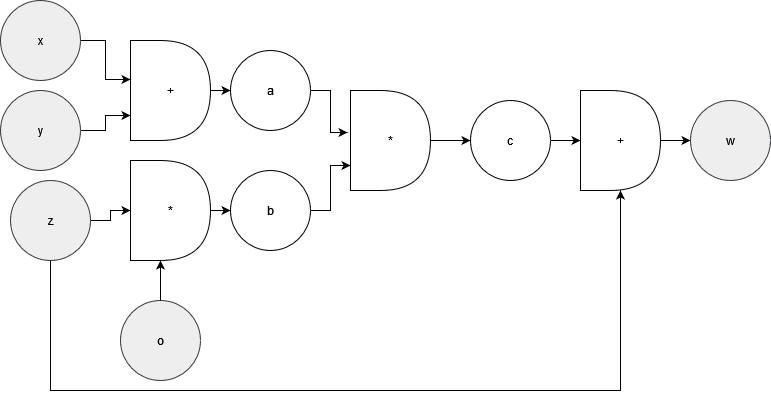
\includegraphics[width=15cm]{diagram2.png}

        \newpage

  \item Draw the graph of the following (and its derivative):
        \begin{enumerate}
          \item ReLU()
                \begin{tcolorbox}
                  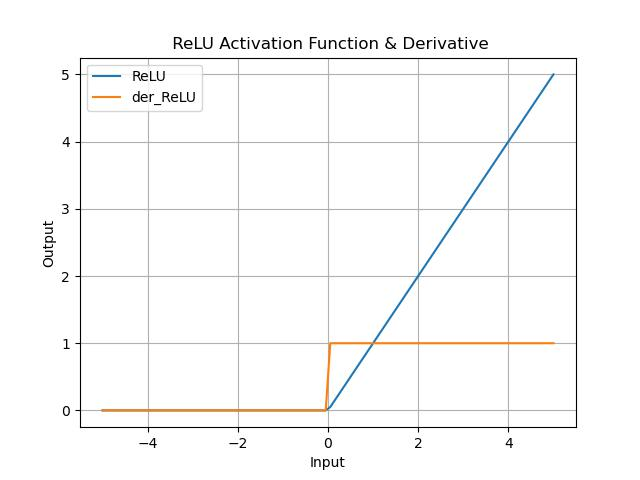
\includegraphics[width=9.5cm]{relu.jpg}
                \end{tcolorbox}
          \item LeakyReLU(0.01)
                \begin{tcolorbox}
                  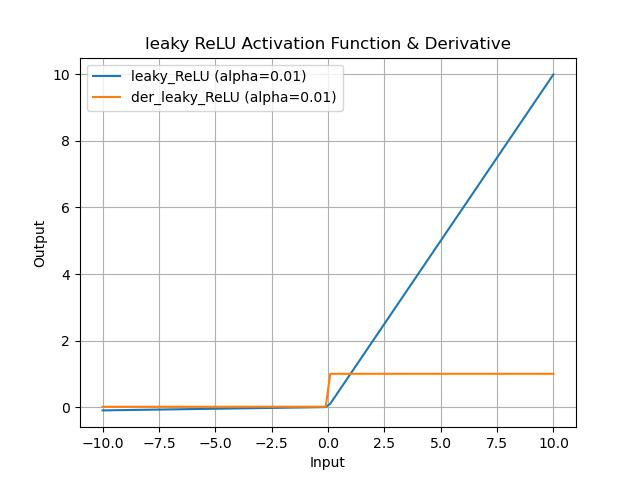
\includegraphics[width=9.5cm]{leaky_relu.jpg}
                \end{tcolorbox}

          \item Softplus(beta is 1)
                \begin{tcolorbox}
                  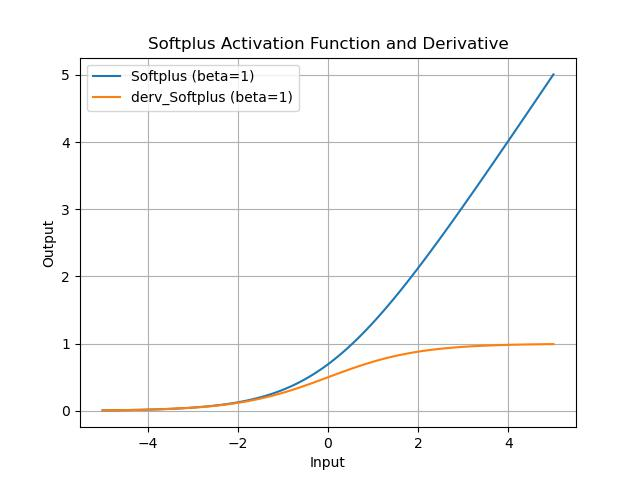
\includegraphics[width=9.5cm]{softplus.jpg}
                \end{tcolorbox}
          \item GELU
                \begin{tcolorbox}
                  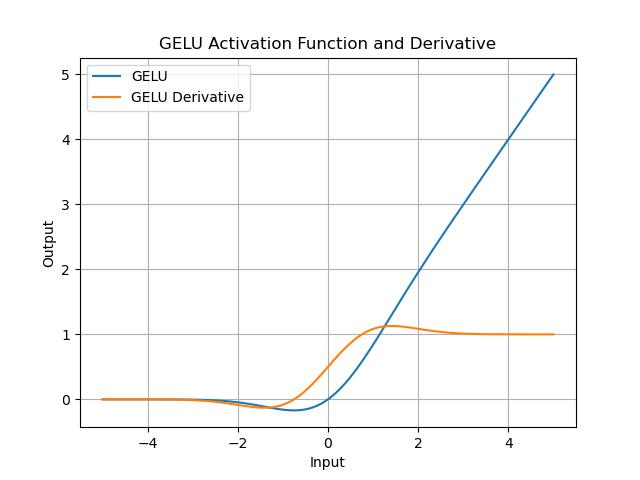
\includegraphics[width=9.5cm]{gelu.jpg}
                \end{tcolorbox}
        \end{enumerate}

        \newpage

  \item (3pt) Explain what are the limitations of the ReLU activation function. How do leaky ReLU and softplus address some of these problems? \\
  \begin{tcolorbox}
    There is the issue of dead neurons when using the ReLU activation function.  If a large gradient flows through a ReLU neuron, 
    it updates weights such that the neuron will always output zero, which prevents any stops learning as no input will be considered. Note that its output is also unbounded.
    To address these concerns the leaky ReLU and softplus prevents dying neurons by introducing non-zero, constant gradient for negative inputs in the case of the former
    and offers a smooth, differentiable alternative that has natural bounds with the latter.
  \end{tcolorbox}

  \item (2pt) What are 4 different types of linear transformations? What is the role of linear transformation and non linear transformation in a neural network?
  \begin{tcolorbox}
    Reflection, rotation, scaling, and shear are the main types of
    linear transformations. In neural networks, each output unit produces the
    linear combination of the inputs and the connection weights. Once we allow
    translation, these essentially become affine transformations. To introduce
    nonlinearity to the model (to capture greater complexity by having a larger hypothesis space), activation functions ingest these transformations
    through a nonlinear function and treat that as the unit output.
  \end{tcolorbox}

\end{enumerate}

%%%%%%%%%%%%%%%%%%%%%%%%%%%%%%%%%%%%%%%%%%%%%%%%%%%%%%%%%%%%%%%%%%%%
%%%%%%%%%%%%%%%%%%%%%%%%%%%%%%%%%%%%%%%%%%%%%%%%%%%%%%%%%%%%%%%%%%%%
%%%%%%%%%%%%%%%%%%%%%%%%%%%%%%%%%%%%%%%%%%%%%%%%%%%%%%%%%%%%%%%%%%%%
\section{Implementation (50pt)}

\subsection{Backpropagation (35pt)}
You need to implement the forward pass and backward pass for $\texttt{Linear}$,
$\texttt{ReLU}$, $\texttt{Sigmoid}$, $\texttt{MSE loss}$, and $\texttt{BCE
    loss}$ in the attached $\texttt{mlp.py}$ file. We provide three example test
cases $\texttt{test1.py}$, $\texttt{test2.py}$, $\texttt{test3.py}$. We will
test your implementation with other hidden test cases, so please create your
own test cases to make sure your implementation is correct.

\textbf{Recommendation}: Go through this \href{https://pytorch.org/tutorials/beginner/basics/intro.html}{Pytorch tutorial} to have a thorough understanding of Tensors.

Extra instructions:
\begin{enumerate}
  \item Please use Python version $\geq 3.7$ and PyTorch version $> 1.7.1$ (this code
        is tested on PyTorch version $2.4.0$). We recommend you to use Miniconda the
        manage your virtual environment.
  \item We will put your $\texttt{mlp.py}$ file under the same directory of the hidden
        test scripts and use the command $\texttt{python hiddenTestScriptName.py}$ to
        check your implementation. So please make sure the file name is
        $\texttt{mlp.py}$ and it can be executed with the example test scripts we
        provided.
  \item You are not allowed to use PyTorch autograd functionality in your
        implementation.
  \item Be careful about the dimensionality of the vector and matrix in PyTorch. It is
        not necessarily follow the the Math you got from part 1.
\end{enumerate}

\subsection{Gradient Descent (15pt + 5pt)}

In DeepDream, the paper claims that you can follow the gradient to maximize an
energy with respect to the input in order to visualize the input. We provide
some code to do this. Given a image classifier, implement a function that
performs optimization on the input (the image), to find the image that most
highly represents the class. You will need to implement the
$\texttt{gradient\_descent}$ function in $\texttt{sgd.py}$. You will be graded
on how well the model optimizes the input with respect to the labels.

Extra hints:
\begin{enumerate}
  \item We try to \emph{minimize} the energy of the class, e.g. maximize the class
        logit. Make sure you are following the gradient in the right direction
  \item A reasonable starting learning rate to try is 0.01, but depending on your
        implementation, make sure to sweep across a few magnitudes.
  \item Make sure you use $\texttt{normalize\_and\_jitter}$, since the neural network
        expect a normalized input. Jittering produces more visually pleasing results
\end{enumerate}

You may notice that the images that you generate are very messy and full of
high frequency noise. Extra credit (5 points) can be had by generating visually
pleasing images, and experimenting with visualizing the middle layers of the
network. There are some tricks to this:
\begin{enumerate}
  \item Blur the image at each iteration, which reduces high frequency noise
  \item Clamp the pixel values between 0 and 1
  \item Implement weight decay
  \item Blur the gradients at each iteration
  \item Implement gradient descent at multiple scales, scaling up every so often
\end{enumerate}

\end{document}
